% \documentclass[bwprint]{cumcmthesis} %去掉封面与编号页
\documentclass[withoutpreface,bwprint]{cumcmthesis} %去掉封面与编号页
\newcommand{\diff}{\mathop{}\!\mathrm{d}} % 正体微分符号

\usepackage{graphicx}       % 用于插入图片
\usepackage{subcaption} 
\usepackage{algorithm}
\usepackage{algorithmic} % 导言区需添加这两个宏包
\usepackage{comment}  

\usepackage{booktabs}
\usepackage{tabularx}
\usepackage{float}
\usepackage[numbers]{natbib}

\title{基于长短期记忆网络(LSTM)的蔬菜补货与定价决策模型}
\tihao{A}
\baominghao{1234}
\schoolname{XX大学}
\membera{yby}
\memberb{hyx}
\memberc{ssh}
\supervisor{老师}
\yearinput{2025}
\monthinput{08}
\dayinput{29}


\begin{document}

% 标题
\maketitle
\nocite{*}
\bibliographystyle{gbt7714-numerical}

\begin{abstract}
本文

    \textbf{针对问题一,}
你好

    \textbf{针对问题二,}

    \textbf{针对问题三,}

    \textbf{针对问题四,}

    \keywords{'xx'\quad'xx'\quad'xx'\quad'xx'\quad'xx'}
\end{abstract}

% 问题背景与重述
\section{问题重述}

\subsection{问题背景}
在无人机集群遂行编队飞行任务时,为降低外界干扰、维持电磁静默状态,拟采用纯方位无源定位技术来调整无人机的位置。该技术的核心是:由编队内部分无人机发射信号,其余无人机被动接收信号,并从接收的信号中提取方向信息以实现定位,进而完成位置调整。编队中的每架无人机都有唯一且固定的编号,且在编队里与其他无人机的相对位置关系保持稳定。

\subsection{问题提出}
接收信号的无人机所获取的方向信息,定义为该无人机与任意两架发射信号无人机连线之间的夹角(示意图可参考图 1)。比如,当编号为 FY01、FY02、FY03 的无人机发射信号时,编号为 FY04 的无人机接收到的方向信息为 \(\alpha_1\)、\(\alpha_2\) 和 \(\alpha_3\)。基于此,需建立数学模型解决以下问题:

\textbf{问题一:}
编队由 10 架无人机组成圆形编队,其中 9 架无人机(编号为 FY01 至 FY09)均匀分布在某一圆周上,另外 1 架无人机(编号 FY00)位于该圆的圆心。所有无人机依靠自身感知的高度信息,保持在同一高度飞行。

\begin{enumerate}
    \item 当位于圆心的无人机(FY00)以及编队中的另外 2 架无人机发射信号,且这 2 架发射信号的无人机位置无偏差、编号已知时,建立被动接收信号无人机(位置存在偏差)的定位模型。
    \item 某位置存在偏差的无人机,能接收到编号为 FY00 和 FY01 的无人机发射的信号,同时还能接收到编队中若干编号未知的无人机发射的信号。要求给出在发射信号的无人机位置均无偏差的情况下,除 FY00 和 FY01 外,需要多少架无人机发射信号能实现该无人机的有效定位。
    \item 按编队要求,1 架无人机位于圆心,另 9 架无人机均匀分布在半径为 $100m$ 的圆周上。当初始时刻无人机的位置略有偏差时,要求给出合理的无人机位置调整方案,即通过多次调整,每次选择编号为 FY00 的无人机和圆周上最多 3 架无人机遂行发射信号,其余无人机根据接收到的方向信息,调整到理想位置,使得 9 架无人机最终均匀分布在某个圆周上。
\end{enumerate}

\textbf{问题二:}
在实际飞行场景中,无人机集群也可采用其他编队队形,例如锥形编队,直线上相邻两架无人机的间距相等。在仍采用纯方位无源定位的情况下,设计无人机的位置调整方案。

% 问题分析
\section{问题分析}

\subsection{问题一分析}
该问题的本质是一个简单的几何求解过程,根据圆上一点的任意性固定一个点同时假设另一点的极坐标,利用方向信息和正弦定理求解被动机的位置,考虑到被动机和圆上主动机的位置关系,可以分为两种情况求解,同时为了简化模型求解,方便计算,设定主动机与被动机的角度范围求出其在一般情况下的解,再根据我们假设的发射信号的先后顺序确定我们所需要的无人机位置的解,从而实现对无人机的有效定位。

\subsection{问题二分析}
该问题先利用圆上相同弦长所对应的圆周角相等的性质,证明出已知两个点及与一个未知点的夹角可以确定该未知点的轨迹为两端圆弧,再利用第三个已知点的位置与该未知点的夹角确定该未知点的位置,从而求解出该未知点的位置。再将此证明结论应用于问题二中即可实现对问题的求解,便可证明只需再有一架主动机即可实现对被动机的有效定位。

\subsection{问题三分析}
该问题本质上是一个局部最优化的问题,先通过对已知数据进行预处理来缩小误差后,分两种方案建立最优化模型,即圆心加圆上两架或三架无人机来发射信号实现无人机阵列调整,构建目标函数来衡量其与实际位置的偏离程度,求目标函数最小值同时记录每架无人机的目标函数来构建误差衡量函数,最后比较两方案的误差以及发射信号的次数来比较方案的优劣来确定选取方案,并通过计算机初始位置生成随机数的模拟来验证。

\subsection{问题四分析}
本题可以根据锥形群的几何特征,通过一些关于几何关系的简单利用来不断调整其位置的直至调整完成,考虑到正三角形的几何性质,提出三种独立的调整策略:保证每个小三角形是正三角形,且点与点之间共线:保证大三角形边上每个点等分:保证中间三角形中心准确。因此,可以基于此假设并证明三条引理,即给定空间中近似成正三角形的三个点与一在其中一边附近的点,可通过将其调整为严格的正三角形:可以将点调至共线并使之成为定比分点:在三角形中心附近的点可通过微调使其成为其中心。随后将15个点分成三类,逐步调整。进行计算机的仿真模拟微小量的调整,随机生成初始数据,并分别计算三个引理所对应的误差值与锥形阵列全局的误差值(通过三维平面拟合求误差平方和),评价模型的优劣性。
% 模型假设
\section{模型假设}

\begin{enumerate}
    \item 假设无人机知道自己的编号。
    \item 假设无人机主动机发射信号有次序,不是同时发射。
    \item 假设无人机调整方向为任意的。
\end{enumerate}

% 符号说明
\section{符号说明}
\begin{table}[H]
    \centering
    \caption{模型核心符号说明}
    \label{表标签}
    \begin{tabular}{ccc} 
        \toprule[1.5pt]
        \textbf{符号} & \textbf{说明} & \textbf{单位} \\
        \midrule[1pt]
        $g$ & 品类标识 & - \\
        $n_g$ & 第$g$类品类的样本量 & - \\
        \bottomrule[1.5pt]
    \end{tabular}
\end{table}

% 模型建立与求解
\section{模型建立与求解}
\subsection{问题一的模型建立与求解}


根据题意,先以FY00作为圆心,FY00与FY01连线方向为极轴,逆时针为正方向建立极坐标。在该极坐标下进行几何求解,位于圆心的无人机FY00和编队中另 2 架无人机发射信号,由于圆上第一架无人机选取具有任意性,为简化模型,方便计算,以FY01为一架主动机,选取其他任意一架无人机作为主动机,发射信号的无人机位置无偏差且编号已知,可由此确定被动机的位置。

\subsubsection{被动机定位模型建立}

根据我们建立的极坐标系,$R$为九架无人机分布圆的半径,可知FY00和FY01的极坐标分别为$(0,0)$,$(R,0)$,设另一架主动机$i$的极坐标为$(R,\theta)$,其中$\theta$已知,设接收信号的被动机$j$极坐标为$(r,\varphi)$,其中$(r)$与$(\varphi)$均未知。根据题意可知接收信号的被动机位置有如下两种情况:

\begin{enumerate}
    \item 当$\theta>\varphi$时,无人机分布的其中一种情况如图\ref{q1_1}所示,

    由几何关系可得
    \begin{equation}
    \left\{
    \begin{aligned}
        \frac{R}{\sin\alpha} &= \frac{r_1}{\sin(\pi - \alpha - \theta + \varphi_1)} \\
        \frac{R}{\sin\beta} &= \frac{r_1}{\sin(\pi - \varphi_1 - \beta)}
    \end{aligned}
    \right.
    \label{式1}
    \end{equation}

    \item 当$\theta<\varphi$时,无人机分布的其中一种情况如图\ref{q1_2}所示,
    
    由几何关系可得
    \begin{equation}
    \left\{
        \begin{aligned}
            \frac{R}{\sin\alpha} &= \frac{r_2}{\sin(\pi - \alpha + \theta - \varphi_2)} \\
            \frac{R}{\sin\beta} &= \frac{r_2}{\sin(\pi - \varphi_2 - \beta)}
        \end{aligned}
    \right.
    \label{式2}
    \end{equation}
    
\end{enumerate}


实际上我们要考虑$\theta$与$\varphi$有四种取值范围,$\theta \in[0,\pi)\cap \varphi \in[0,\pi)$,$\theta \in[0,\pi)\cap \varphi \in[\pi,2\pi)$,$\theta \in[\pi,2\pi)\cap \varphi \in[0,\pi)$,$\theta \in[\pi,2\pi)\cap \varphi \in[\pi,2\pi)$四种情况。易证$\theta$与$\varphi$的取值范围不影响数值解的大小,仅影响解的正负,故仅从$\theta$与$\varphi$的大小关系出发进行讨论。上述描述便以$\theta \in[0,\pi]\cap \varphi \in[0,\pi)$为例,其他情况均同理。


\begin{figure}[H]
    \centering
    \begin{minipage}{0.49\textwidth}
        \centering
        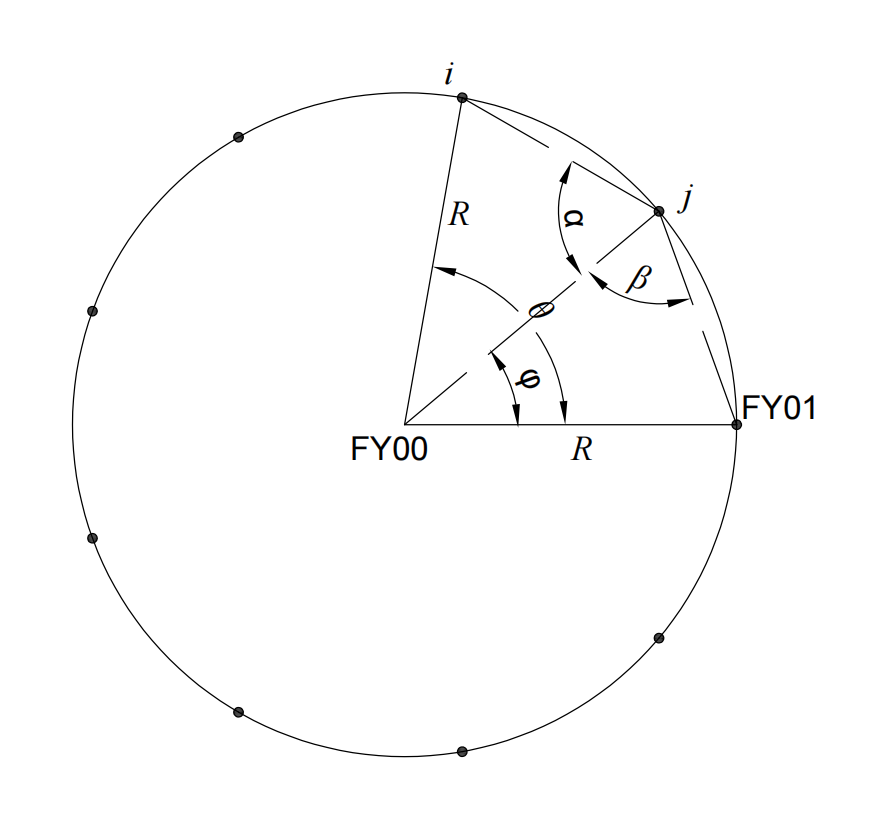
\includegraphics[width=0.9\textwidth]{../../figure/q1_1.png} 
        \caption{主动机与被动机排布的情况1}
        \label{q1_1}
    \end{minipage}
    \begin{minipage}{0.49\textwidth}
        \centering
        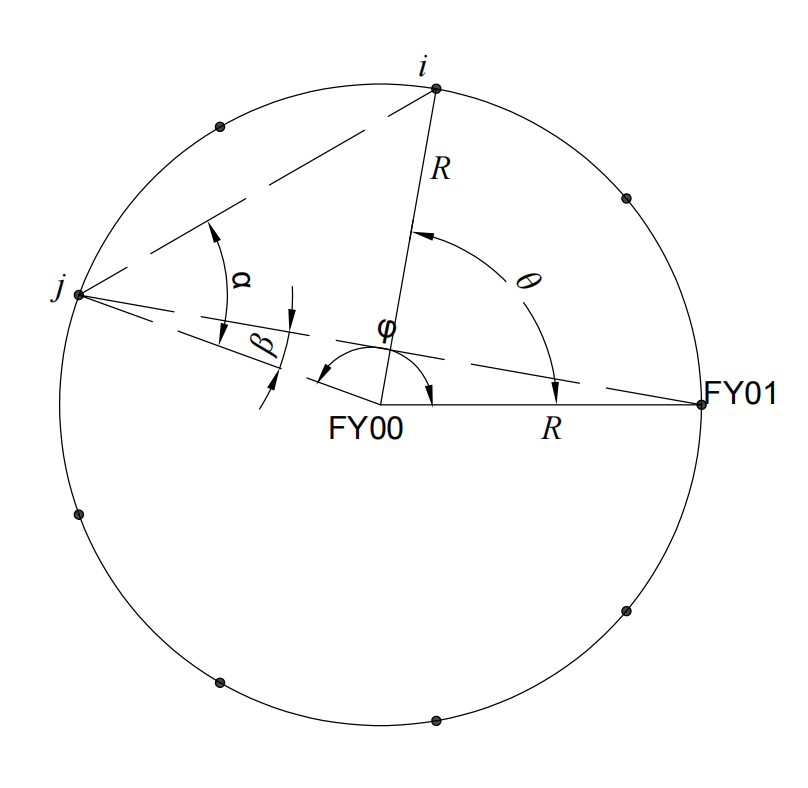
\includegraphics[width=0.86\textwidth]{../../figure/q1_2.png} 
        \caption{主动机与被动机排布的情况2}
        \label{q1_2}   
    \end{minipage}
    \caption*{\small 注:主动机发射的方向信息$\alpha$为$(i,0)$的夹角,$\beta$为$(0,1)$的夹角。}
\end{figure}



\subsubsection{被动机定位模型求解}

进行情况一$\theta>\varphi$的求解,将式(\ref{式1})相除可得

\begin{equation}
    \frac{\sin\beta}{\sin\alpha} = \frac{\sin(\pi - \varphi_1 -\beta)}{\sin(\pi - \alpha - \theta + \varphi_1)}
\end{equation}

将上式整理得

\begin{equation}
    \tan\varphi_1= \frac{\cos\alpha + \cos(\beta +\theta)}{\sin(\alpha+\theta)- \sin\beta}
\end{equation}

则上述方程的解为

\begin{equation}
    \left\{
        \begin{aligned}
            \varphi_1 &= \arctan \frac{\cos\alpha+\cos(\beta+\theta)}{\sin\alpha[\sin(\beta+\theta)-\sin\beta]} \\
            r_1 &= \frac{R \sin(\beta-\varphi_1+\theta)}{\sin\beta}
        \end{aligned}
    \right.
    \label{解1}
\end{equation}

同理,对情况二$\theta<\varphi$求解可得

\begin{equation}
    \left\{
        \begin{aligned}
            \varphi_2 &= \arctan \frac{\cos\alpha-\cos(\beta-\theta)}{\sin\alpha[\sin(\beta-\theta)-\sin\beta]} \\
            r_2 &= \frac{R \sin(\beta-\varphi_2-\theta)}{\sin\beta}
        \end{aligned}
    \right.
\end{equation}

在求解过程中,我们得到被动机位置的极坐标解为\((r_1,\varphi_1)\)和\((r_2,\varphi_2)\)。在几何上关于三架主动机对应圆心角的角平分线对称分布(见图\ref{q1_3})。特别地,当被动机位于该角平分线的延长线上时,两个解将重合(见图\ref{q1_4})。

\begin{figure}[H]
    \centering
    \begin{minipage}{0.49\textwidth}
        \centering
        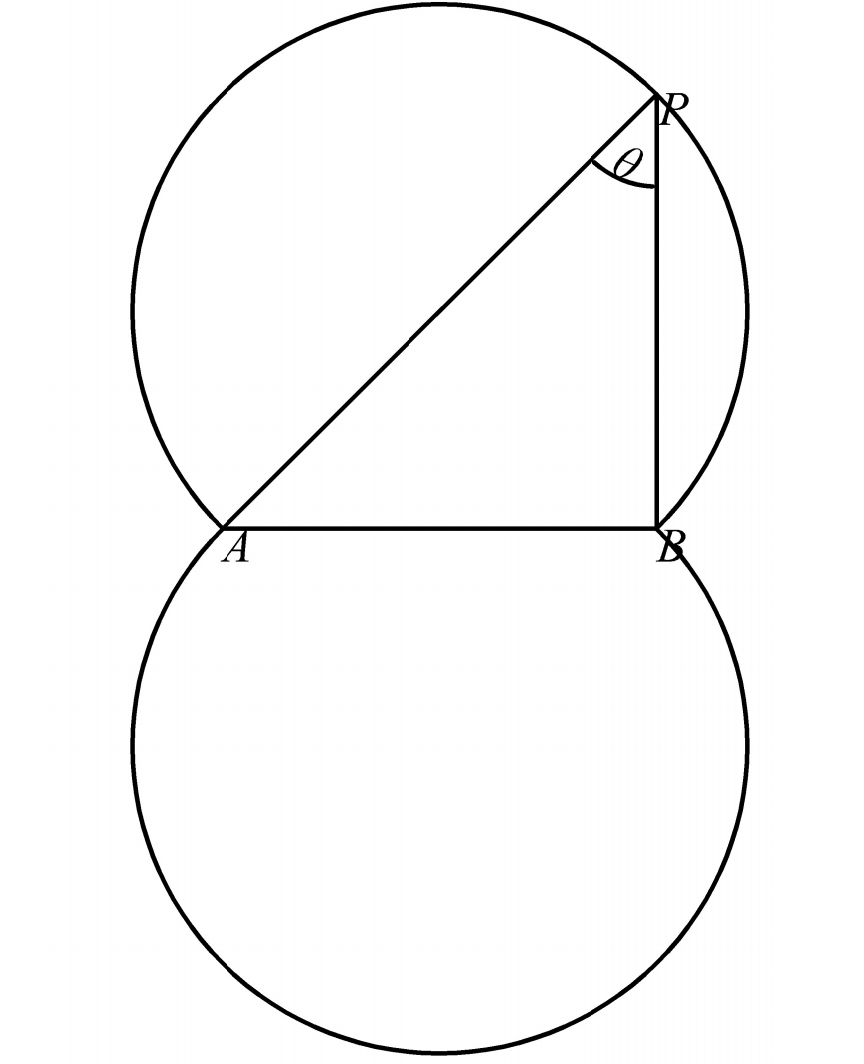
\includegraphics[width=0.9\textwidth]{../../figure/q1_3.png} 
        \caption{两组解的对称分布示意图}
        \label{q1_3}
    \end{minipage}
    \begin{minipage}{0.49\textwidth}
        \centering
        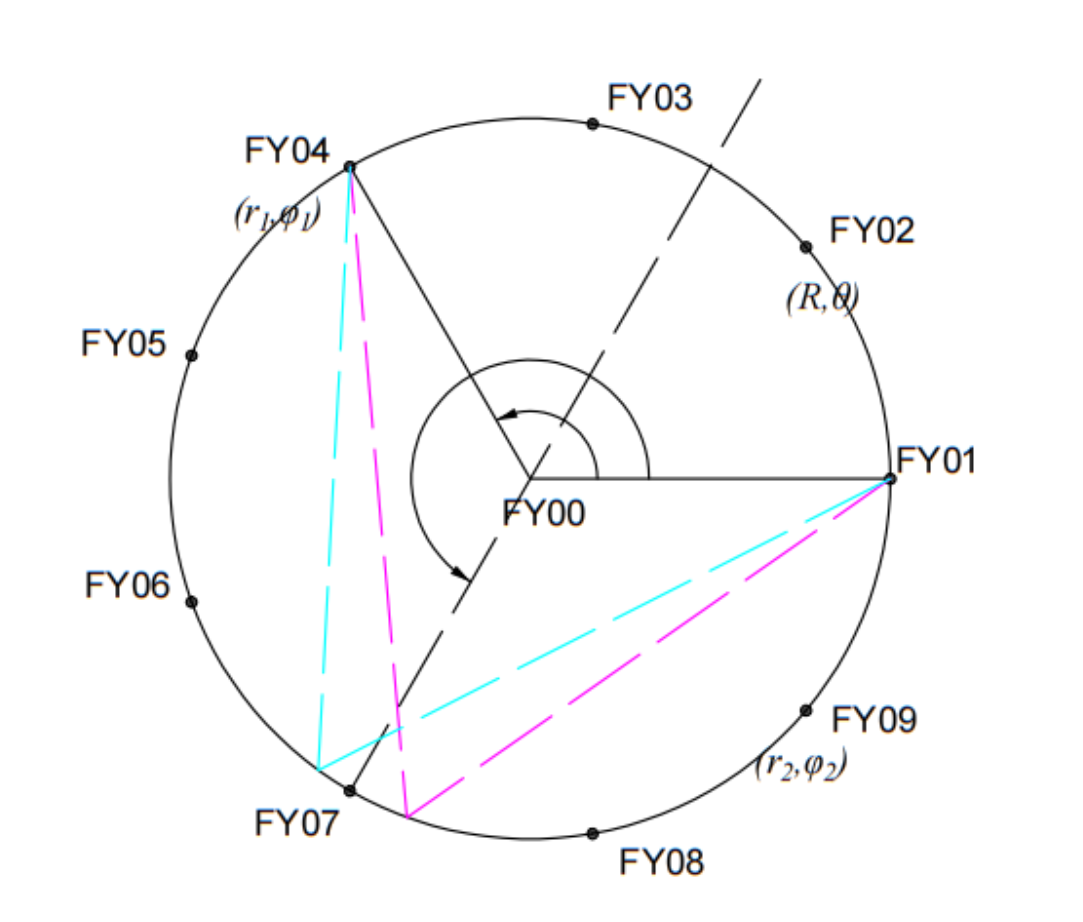
\includegraphics[width=0.86\textwidth]{../../figure/q1_4.png} 
        \caption{解的重合情况示意图}
        \label{q1_4}   
    \end{minipage}
\end{figure}


由于无法直接确定\(\alpha\)、\(\beta\)分别对应哪两台主动机发射的信号,因此会产生两个可能的位置解。为确定实际位置,假设主动机信号的发射次序已知,被动接收信号的无人机已知自身对应的编号,这一假设在实际场景中具有合理性。

以图 \ref{q1_4} 为例,FY07 为被动机,FY00、FY04、FY01 为主动机。当被动机位置存在微小偏差时,$\alpha$与$\beta$近似相等。由于传感器的无源特性,FY07 仅能接收方向信息,无法识别$\alpha$和$\beta$对应的主动机编号,因此可能位于图中的 M、N 两点。

为排除虚假位置、确定真实位置,可利用信号源的非同步发射特性 —— 假设信号发射存在时间次序,那么 FY07 接收的信号将具有时序特征。基于这一特征可识别$\alpha$和$\beta$对应的主动机,从而唯一确定被动机的实际位置。


\subsection{问题二的模型建立与求解}
为确定在已知FY00和FY01为无偏差的主动机的前提下,确定还需要几架主动机可以实现对被动机的有效定位,我们先证明一个引理:得出已知三点及两个与未知点的夹角可以确定该点的位置。基于次引理可再证明只需再加一架主动机便可实现对被动机的有效定位。
\subsubsection{模型建立}
引理的证明:假定我们已知点A,B的位置以及与未知点P的夹角$\theta$,我们可以通过几何关系得出点P的轨迹为以AB为弦的两端圆弧,如图\ref{q2_1}所示即为点P的轨迹。接下来我们再引入点U,已知PU与PB的夹角$\beta$,我们可以通过几何关系得出点P的轨迹为以BU为弦的两端圆弧。由此可得出点P两个轨迹的交点即为点P的确切位置,P的具体位置如图\ref{q2_2}所示。至此,证毕。

\begin{figure}[H]
    \centering
    \begin{minipage}{0.49\textwidth}
        \centering
        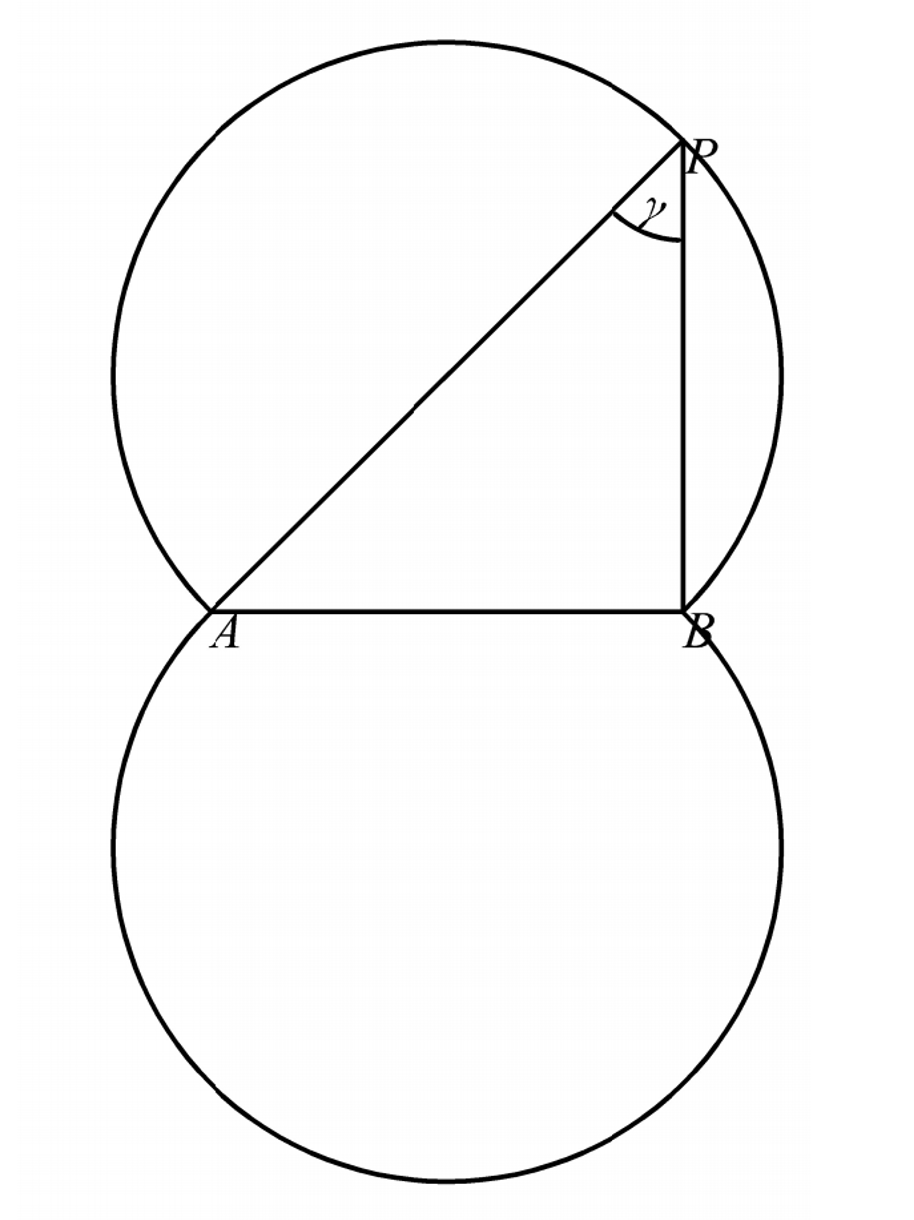
\includegraphics[width=0.75\textwidth]{../../figure/q2_1.png} 
        \caption{主动机与被动机排布的情况1}
        \label{q2_1}
    \end{minipage}
    \begin{minipage}{0.49\textwidth}
        \centering
        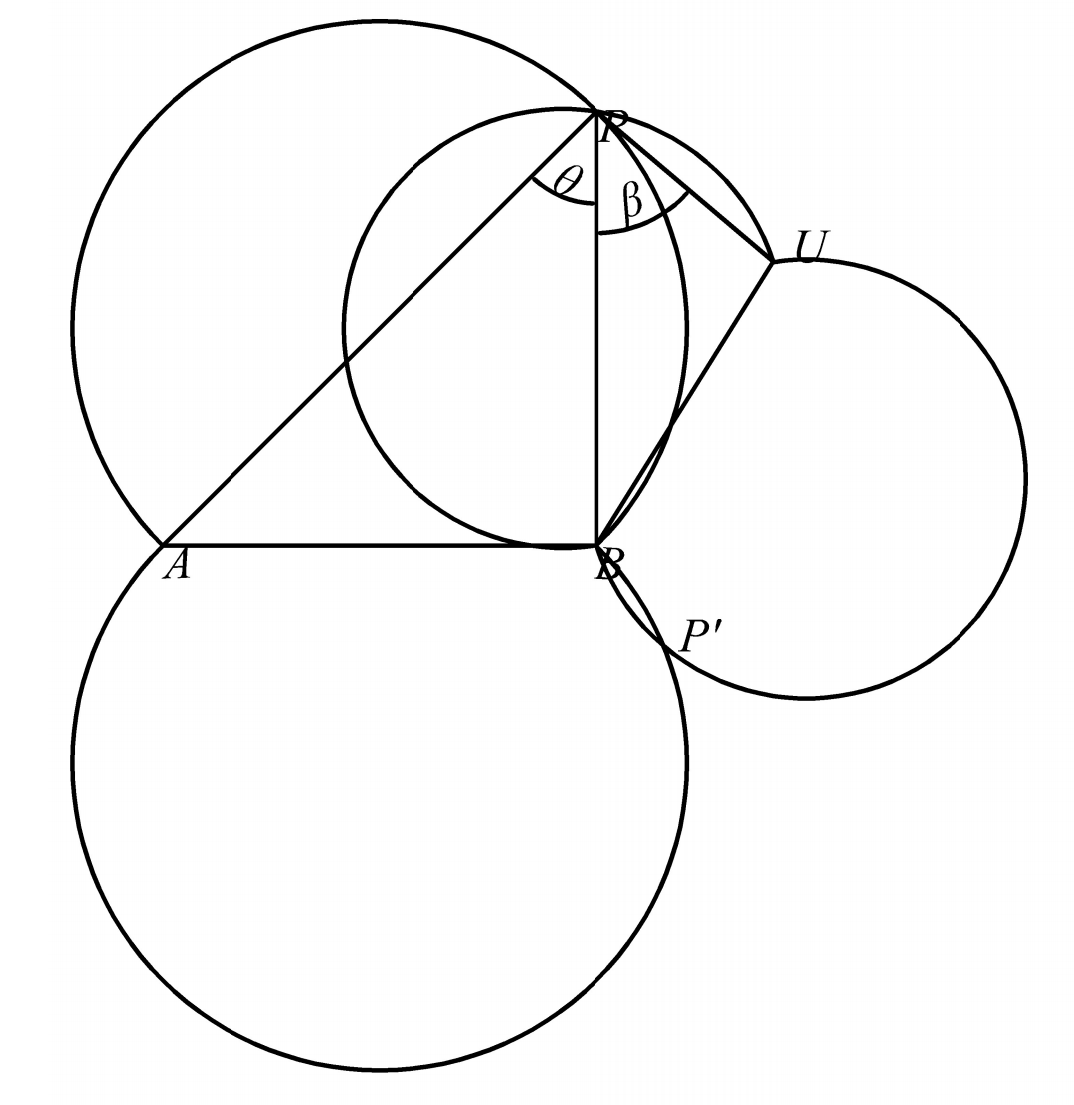
\includegraphics[width=0.9\textwidth]{../../figure/q2_2.png} 
        \caption{主动机与被动机排布的情况2}
        \label{q2_2}   
    \end{minipage}
\end{figure}

\subsubsection{问题求解}
我们把引理代入到本题中,已知FY00和FY01为主动机,且与被动机的夹角为发射信号,发射信号已知,因此可以确定被动机的轨迹。接下来引入第三架主动机FY02,已知FY02与FY00或FY01与被动机的夹角,通过几何关系可以确定被动机的确切位置。但根据我们上述证明,P的确切位置有两个,但是由于被动机再圆周上,因此有一个解是无效解,应舍弃。通过次方法我们实现了对无人机的有效定位。



\subsection{问题三的模型建立与求解}
首先对问题中的数据进行预处理,预处理的方法是通过点距离圆心距离与理想位置的对比,将其沿径向调整,以使数据更加接近理想位置的同时,为后续调整减少运算和节约时间。分两种情况建立局部最优模型,构建以方向信息与理想位置的方向信息的差的平方和为目标函数,和以目标函数为和的误差函数,来衡量无人机的调整方案的优劣,最后再通过仿真来验证。

\subsubsection{数据预处理}
由题意可得我们可以得到每个无人机的具体数据,将无人机编号为0,1的无人机定义为此圆心和圆上一点来确定该圆周(即认为该两个点为准确的),通过判断圆上其他无人机的位置与该圆周的关系,来沿径向调整,使其更接近理想位置,调整方法如下:将无人机0,1发射的方向信息调整为$90°-20°(j-1)$,$j$为无人机的编号,如图\ref{q3_1}所示。

\begin{figure}[H]
    \centering
    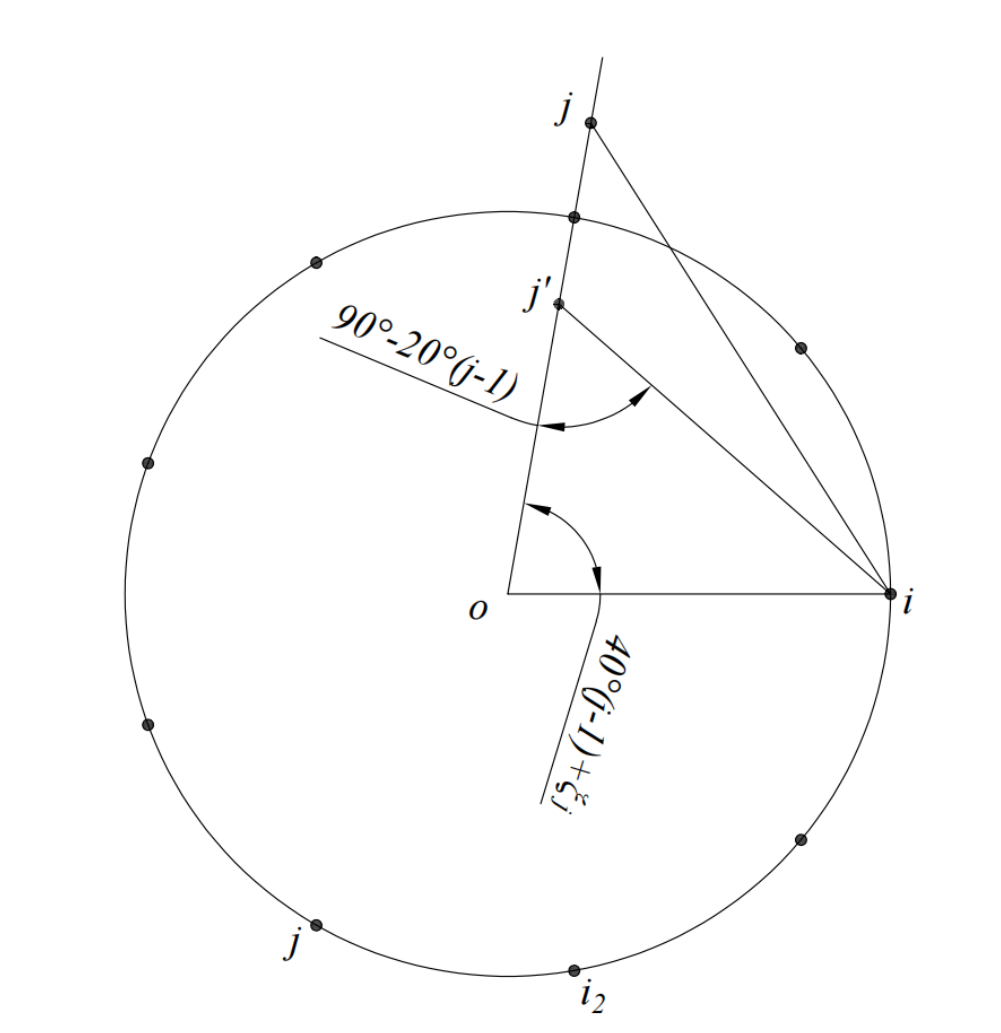
\includegraphics[width=0.6\textwidth]{../../figure/q3_1.png} 
    \caption{无人机位置调整示意图}
    \label{q3_1}    
\end{figure}

\subsubsection{模型建立}

我们一般选取调整方案应当选取最优的调整方案,以节省人力、物力、财力,因此我们应选择两种情况下最优的方案,即发射信号尽可能少,定位精度尽可能高。因此我们建立目标函数来衡量无人机位置与理想位置的偏离程度,建立误差函数来衡量无人机位置的调整精度。根据题意,我们选择圆心和圆上两架或三架无人机发射信号来调整无人机的位置。

\begin{enumerate}
    \item 选取圆心和圆上两个为主动机发射信号。
    
        为尽可能平均调整每架无人机的位置,尽可能少的发射信号,我们以此选取027、038、049、015、016,为发射信号的无人机,其余无人机被动接收信号,调整位置。我们建立局部目标函数并求解其最优解,根据局部最优模型做出调整。

        \textbf{Step1:} 选取027为发射信号无人机,1345689无人机被动接受信号并作出调整(1不需要调整)。以无人机9接收信号为例(其余无人机与3大同小异,目标函数见表3),
     
        其调整方式如下:记 $\angle 709 = \alpha$,$\angle 902 = \beta$。由正九边形几何关系易知,$\alpha$,$\beta$ 三个角的理想值均为 $50^\circ$(不同发射信号的无人机,不同接受信号的无人机确切指导见表 \ref{表3})。记 $x = [\alpha, \beta]^T$,$y = [50^\circ, 50^\circ]^T$,建立目标函数
\[
f_9(\alpha, \beta, \gamma) = \Vert{x} - {y}\Vert_2^2 = (\alpha - 50^\circ)^2 + (\beta - 50^\circ)^2
\]
$f_9$ 下标为对应无人机编号。依此,其余待调整无人机目标函数为 $f_3, f_4, f_5, f_6, f_8$。以无人机 9 为中心,在边长为 $a$ 的正方形区域内以步长 $b$ 调整,使目标函数达到最小值。


\begin{table}[htbp]
  \centering
  \caption{目标函数序列}
  \label{表3}
  \begin{tabular}{ccccc}
    \toprule
    & 2 & 3 & 4 & 5 \\
    \midrule
    027 &  & $(70^\circ, 10^\circ)$ & $(30^\circ, 50^\circ)$ & $(30^\circ, 50^\circ)$ \\
    038 & $(70^\circ, 30^\circ)$ &  & $(70^\circ, 10^\circ)$ & $(50^\circ, 30^\circ)$ \\
    049 & $(50^\circ, 50^\circ)$ & $(70^\circ, 30^\circ)$ &  & $(70^\circ, 10^\circ)$ \\
    015 & $(70^\circ, 30^\circ)$ & $(50^\circ, 50^\circ)$ & $(70^\circ, 30^\circ)$ &  \\
    016 & $(70^\circ, 10^\circ)$ & $(50^\circ, 30^\circ)$ & $(50^\circ, 30^\circ)$ & $(70^\circ, 10^\circ)$ \\
    \bottomrule
  \end{tabular}
\end{table}

\begin{table}[htbp]
  \centering
  \caption{目标函数序列续表}
  \label{表4}
  \begin{tabular}{ccccc}
    \toprule
    & 6 & 7 & 8 & 9 \\
    \midrule
    027 & $(70^\circ, 10^\circ)$ &  & $(70^\circ, 30^\circ)$ & $(50^\circ, 50^\circ)$ \\
    038 & $(50^\circ, 30^\circ)$ & $(70^\circ, 10^\circ)$ &  & $(70^\circ, 30^\circ)$ \\
    049 & $(50^\circ, 30^\circ)$ & $(50^\circ, 30^\circ)$ & $(70^\circ, 10^\circ)$ &  \\
    015 & $(70^\circ, 10^\circ)$ & $(50^\circ, 30^\circ)$ & $(50^\circ, 30^\circ)$ & $(70^\circ, 10^\circ)$ \\
    016 &  & $(70^\circ, 30^\circ)$ & $(50^\circ, 50^\circ)$ & $(70^\circ, 30^\circ)$ \\
    \bottomrule
  \end{tabular}
\end{table}

    \textbf{Step2:} 分别选取038、049、015、016为发射信号无人机,其他无人机被动接受信号并作出调整(1不需要调整),调整方式与Step1类似,此处不再赘述。

    \textbf{Step3:} 设置总循环次数为$\sigma$,总调整次数为 $4\sigma \times 2 \times 8 = 64\sigma$ 次,从而若每辆无人机(0,1除外)调整次数超过7,即$\sigma>\frac{n}{4}$,则该飞机调整结束。否则,$\sigma \leq\frac{n}{4}$,返回Step1继续调整。


    \textbf{Step4:} 定义误差检测函数量化无人机趋于正九边形程度
\[
\mu = v_2 + v_3 + v_4 + v_5 + v_6 + v_7 + v_8 + v_9
\]
综上所述,方案二对应的流程图可表示如下图\ref{q3_2}所示。

\begin{figure}[H]
    \centering
    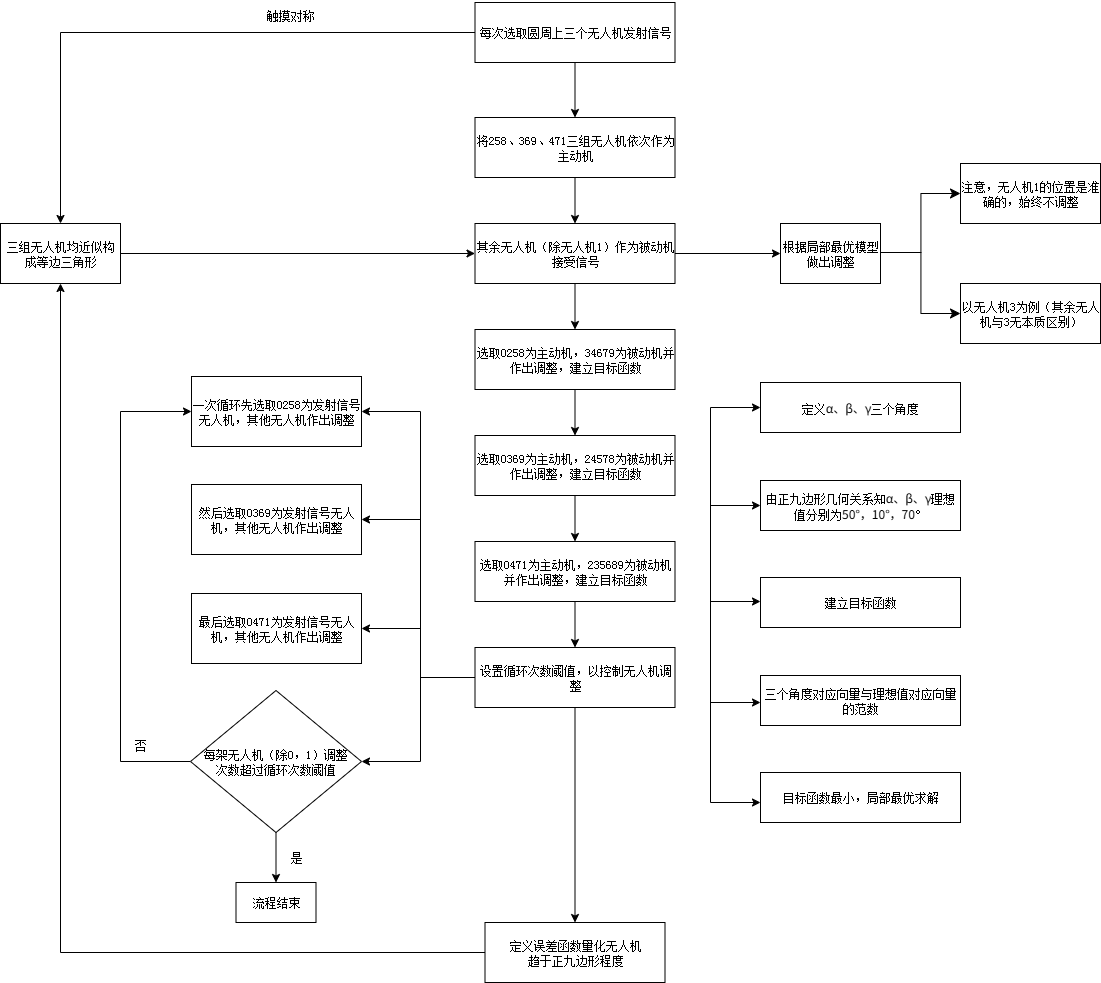
\includegraphics[width=0.95\textwidth]{../../figure/q3_2.png} 
    \caption{方案一对应的流程图}
    \label{q3_2}    
\end{figure}


    \item 选取圆心和圆上三个为主动机发射信号。

考虑正九边形的对称性,258、369、471 三组无人机均近似构成等边三角形,依次将它们作为发射信号的无人机,其余无人机(除无人机 1,其位置准确,始终不调整)接收信号并根据局部最优模型调整位置。

\textbf{Step1:} 选取 0258 为发射信号无人机,134679 无人机被动接受信号并作出调整(1 不需要调整)。以无人机 3 为例(其余无人机与 3 无本质区别),调整方式如下:
记 $\angle 530 = \alpha$,$\angle 038 = \beta$,$\angle 032 = \gamma$。由正九边形几何关系易知,$\alpha$、$\beta$、$\gamma$ 三个角的理想值分别为 $50^\circ$、$10^\circ$、$70^\circ$。记 $x = [\alpha, \beta, \gamma]^T$,$y = [50^\circ, 10^\circ, 70^\circ]^T$,建立目标函数
\[
f_3(\alpha, \beta, \gamma) = \Vert{x} - {y}\Vert_2^2 = (\alpha - 50^\circ)^2 + (\beta - 10^\circ)^2 + (\gamma - 70^\circ)^2
\]
$f_3$ 下标为对应无人机编号。依此,其余待调整无人机目标函数为 $f_4, f_5, f_6, f_7, f_9$。以无人机 3 为中心,在边长为 $a$ 的正方形区域内以步长 $b$ 进行搜索,使目标函数达到最小值。这里设置邻域边长、搜索步长是为了利用 Python 对无人机实际调整进行仿真模拟,实际中无人机可在原来位置附近任意搜索。需要注意的是,此处(包括后续步骤)定义的目标函数为局部函数,仅通过待调整飞机接收到的信息建立,是根据模型假设在已有基础上推断出来的。

\textbf{Step2:} 分别选取 0369、0417 为发射信号无人机,其他无人机被动接受信号并作出调整 (1 不需要调整),调整方式与 Step1 类似,此处不再赘述。

\textbf{Step3:} 设置总循环次数为 $\sigma$,一次循环指先选取 0258 为发射信号无人机,其他无人机作出调整;然后选取 0369 为发射信号无人机,其他无人机作出调整;最后选取 0471 为发射信号无人机,其他无人机作出调整。一次循环中,每架无人机(无人机 0、1 除外)均被一次选做发射信号无人机,且被选做两次被动接受信号无人机并做出调整。若总循环次数为 $\sigma$,总调整次数为 $2\sigma \times 3 \times 8 = 48\sigma$。若每架无人机(0、1 除外)调整次数超过 7,即 $\sigma > \frac{n}{2}$,则该飞机调整结束;否则,$\sigma \leq \frac{n}{2}$,返回 Step1 继续调整。

\textbf{Step4:} 定义误差检测函数量化无人机趋于正九边形的程度
\[
\mu = g_2 + h_2 + g_3 + h_3 + g_4 + h_4 + g_5 + h_5 + g_6 + h_6 + g_7 + h_7 + g_8 + h_8 + g_9 + h_9
\]

综上所述,方案一对应的流程图可表示如下图 \ref{q3_1} 所示。

\begin{figure}[H]
    \centering
    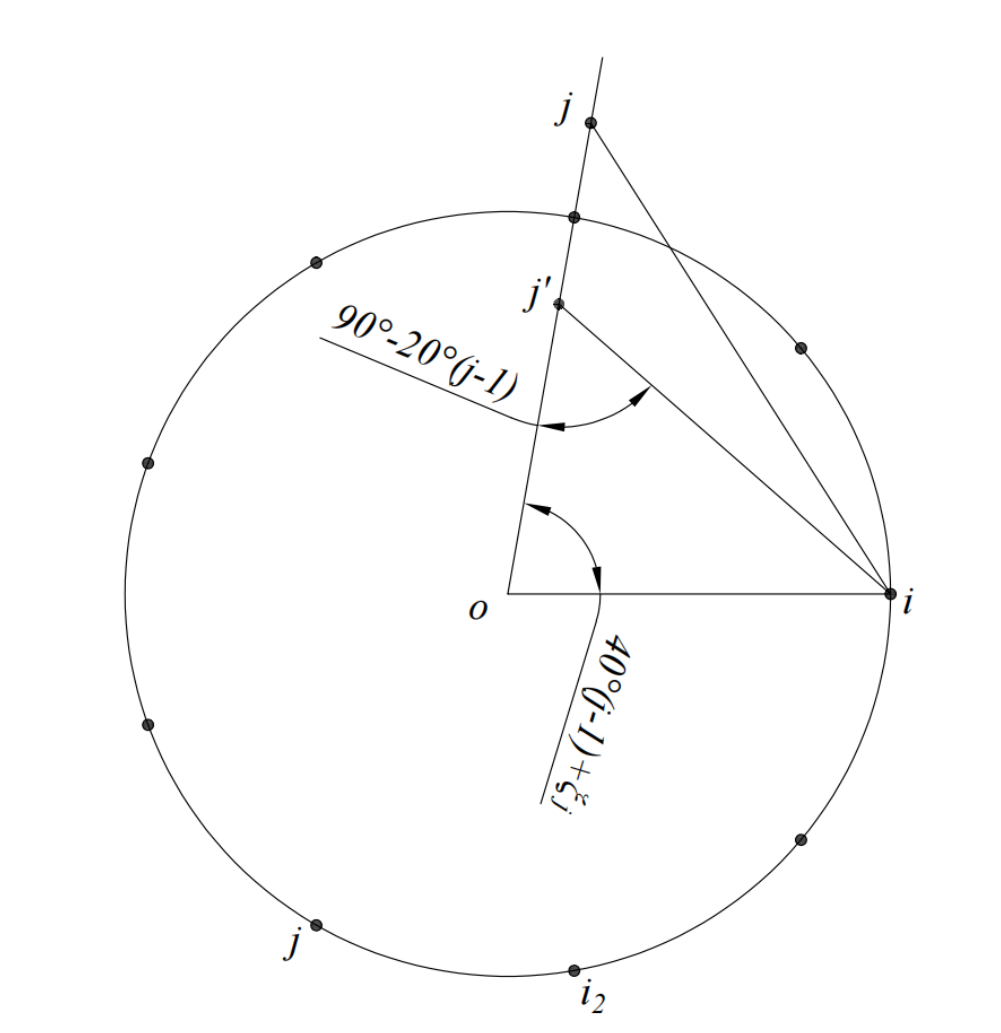
\includegraphics[width=0.95\textwidth]{../../figure/q3_1.png} 
    \caption{方案二对应的流程图}
    \label{q3_1}    
\end{figure}




\end{enumerate}







\subsubsection{问题求解}
\subsubsection{求解结果}


\subsection{问题四的模型建立与求解}
仍考虑纯方位无源定位的情形,设计无人机位置调整方案,我们依然可以使用简单的数学几何关系进行建模。
\subsubsection{模型建立}
\subsection*{引理1}
给定空间中近似为正三角形的三点 \( A, B, C \),以及在边 \( AC \) 附近的一点 \( D \),可通过\textbf{三步微调}将 \( \triangle ABC \) 调整为\textbf{严格正三角形}(调整过程中点 \( B \) 始终不动,且最终 \( D \) 落在边 \( AC \) 上):

\noindent \textbf{第一步:调整点 \( D \)(保持 \( A, B, C \) 不动)}
固定点 \( A, B, C \) 的位置,调整点 \( D \),使 \( \angle ADC = 180^\circ \),从而让 \( D \) 落在边 \( AC \) 上。

\noindent \textbf{第二步:调整点 \( C \)(保持 \( A, B, D \) 不动)}
固定点 \( A, B, D \) 的位置,调整点 \( C \),使 \( \angle ACD = 0^\circ \)(即 \( C \) 落在边 \( AD \) 上),且 \( \angle DCB = \angle BCA = 60^\circ \),从而保证 \( \triangle ABC \) 中 \( \angle C = 60^\circ \)。

\noindent \textbf{第三步:调整点 \( A \)(保持 \( B, D, C \) 不动)}
固定点 \( B, D, C \) 的位置,调整点 \( A \),使 \( \angle CAD = 0^\circ \)(即 \( A \) 落在边 \( CD \) 的延长线上),且 \( \angle DAB = \angle BCA = 60^\circ \),从而保证 \( \triangle ABC \) 中 \( \angle A = 60^\circ \)。

通过上述三步,可在原位置附近将 \( \triangle ABC \) 微调为严格正三角形(记为 \( \triangle AB'C' \)),且最终点 \( D \) 位于边 \( AC \) 上。
\subsection*{引理1}
给定空间中近似成正三角形的三个点\( A,B,C \),与一在边\( AC \)附近的点\( D \),对于任意\( \lambda \in [0, +\infty] \),可以将点调到边\( AC \)上,且满足\( AD/DC = \lambda \)。

当点\( D \)在边\( AC \)上,且满足\( AD/DC = \lambda \)时,根据正三角形几何关系易求
\[
\angle ADB = \arccos \frac{\lambda - 1}{2\sqrt{\lambda^2 + \lambda + 1}}
\]

调整方案如下:点\( A,B,C \)不动,微调点\( D \),控制:
\[
\angle ADC = 0^\circ, \quad \angle ADB = \arccos \frac{\lambda - 1}{2\sqrt{\lambda^2 + \lambda + 1}}
\]
使得点\( D \)在边\( AC \)上且满足\( AD/DC = \lambda \)。
\subsection*{引理3} 
给定空间中成正三角形的三个点\(A,B,C\),与在\(\triangle ABC\)中心附近的点D,可通过微调使得D是\(\triangle ABC\)的中心。点\(A,B,C\)不动,微调点D。控制
\(\angle ADB = \angle BDC = \angle CDA = 120^\circ\)
即可使点D为\(\triangle ABC\)的中心。证明是显然的:由于此时\(\angle ADB + \angle BDC + \angle CDA = 360^\circ\),故点D在平面ABC内;由 F 定理,平面上满足\(\angle ADB = \angle BDC = \angle CDA = 120^\circ\)的点只有一个 —— 费马(FERMAT)点;又因为\(\triangle ABC\)是正三角形,其费马点即为中心,从而点D为\(\triangle ABC\)的中心。
\subsubsection{问题求解}
通过上述三个引理,我们可以利用引理调整阵列使其为严格锥形编队,具体调整流畅如下:
先利用引理1,将最外面三个点调整为正三角形的同时将三角形边上的点调整到边上;然后利用引理2,将边上的点调整为等分点;最后利用引理3,将中间的点调整为三角形的中心。通过上述三步,我们可以将近似锥形阵列调整为严格锥形阵列。至此我们便完成了问题四的理论求解。
\subsubsection{问题四的仿真}
\begin{figure}[H]
    \centering
    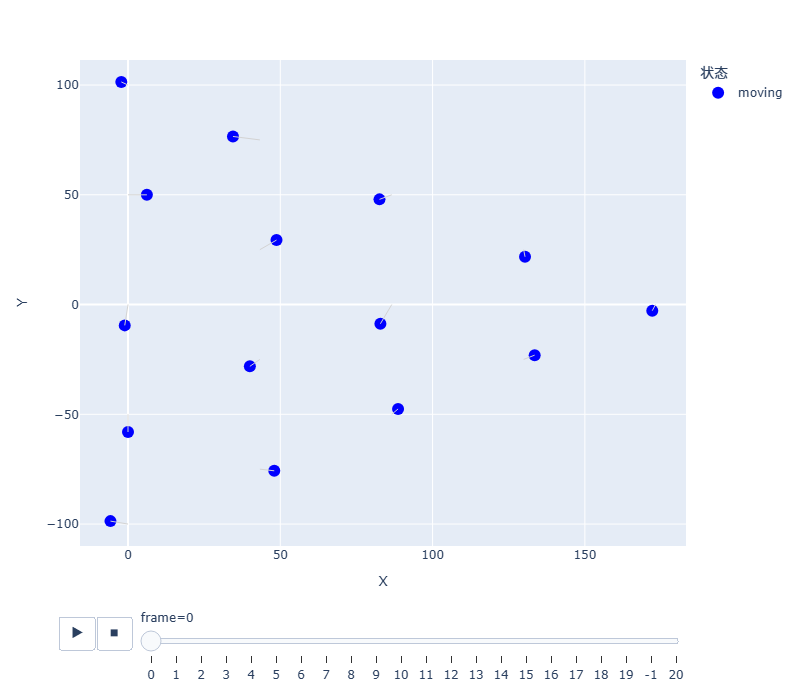
\includegraphics[width=0.85\textwidth]{../../figure/start_4.png} 
    \caption{仿真的初始位置}
    \label{q4_2}    
\end{figure}
\begin{figure}[H]
    \centering
    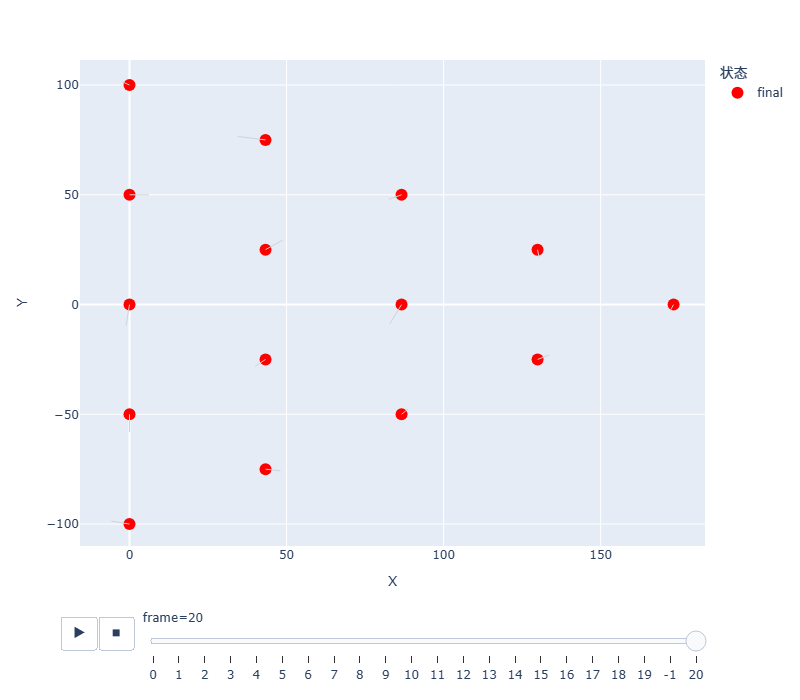
\includegraphics[width=0.85\textwidth]{../../figure/end_4.png} 
    \caption{仿真的初始位置}
    \label{q4_2}    
\end{figure}


% 模型的分析与检验
\section{模型的分析与检验}
\subsection{误差分析}
\subsection{灵敏度分析}


% 模型评价
\section{模型的评价}
\subsection{模型优点}
\begin{enumerate}
    \item 通过简单的数学几何关系求解出问题一的被动机位置,数据结果较准确。
    \item 模型推广性强,生活中除无人机,还有军事侦查、海上侦查、北斗卫星均适用。
    \item 问题二的通过数学几何知识调整可以使锥形队伍调整便捷迅速。
\end{enumerate}

\subsection{模型缺点}
\begin{enumerate}
    \item 没有考虑环境因素对信号传播的影响,如多径效应、信号衰减等。
    \item 模型假设主动机与被动机之间的距离较近,未考虑大范围场景下的定位问题。
\end{enumerate}

\subsection{改进方向}
\begin{enumerate}
    \item 引入环境因素的影响模型,如多径效应、信号衰减等,以提高定位精度。
    \item 增加主动机与被动机之间的距离限制,以适应大范围场景下的定位需求。
\end{enumerate}

% 摘要
\bibliography{ref}

% 附录

\begin{appendices}

\section{运行结果}


\section{文件列表}
\begin{table}[H]
    \caption{程序文件列表}
    \centering
    \begin{tabularx}{\textwidth}{l X}
        \bottomrule
        文件名 & 功能描述 \\
        \midrule
        Calculator.py & 计算工具集合(如计算两点距离等) \\
        Draw.py & 绘图工具 \\
        FindPointBy3P3A.py & 求解三点三角对应点坐标 \\
        code1.py & 问题一程序代码 \\
        code2.py & 问题二程序代码 \\
        code3.py & 问题三程序代码 \\
        code3.py & 问题四程序代码 \\
        \bottomrule
    \end{tabularx}
    \label{tab:文件列表}
\end{table}

\section{代码}
计算工具集合
\lstinputlisting[language=python]{../../code/Calculator.py}
绘图工具
\lstinputlisting[language=python]{../../code/Draw.py}
求解三点三角对应点坐标
\lstinputlisting[language=python]{../../code/FindPointBy3P3A.py}
问题四
\lstinputlisting[language=python]{../../code/code4.py}

\end{appendices}

\end{document}